
\noindent ключением некоторых особых моментов, оно потребует не очень много объяснений.
\begin{lstlisting}[mathescape=true, language=Ada, basicstyle=\small]
function Dichotomic_Exponentiation (x0 : Monoid_Element; n0 : Exponent)
$\qquad$ $\quad$ return Monoid_Element is

begin
$\quad$ if n0 < 0 then raise Numeric_Error; end if;
$\quad$ Calculate_x_Power_n : declare
$\quad$ x : Monoid_Element := x0;
$\quad$ n : Exponent := n0;
$\quad$ Correction : Monoid_Element;

begin
$\quad$ if n mod 2 /= 0 then Correction := x;
$\quad$ else Correction := Monoid_Unit;
$\quad$ end if;

loop
$\quad$ n := n / 2  ${\bf -- Correction * (x ** 2) ** n = x0 ** n0}$
exit when n = 0;
$\quad$ x := x * x;
$\quad$ if n mod 2 /= 0 then Correction := Correction * x; end if;
end loop;

$\quad$ return Correction;
end Calculate_x_Power_n;
end Dichotomic_Exponentiation;

\end{lstlisting}
 
 \par Первое замечание по тексту программы касается обработки одной из ошибок использования, отмеченной в начале этого раздела: использование функции с отрицательным показателем. Эта ошибка легко поддаётся обраружению, и о ней несложно сообщить: для этого используют один из сильных моментов языка Ада, обработку исключений. Команn $\blacktriangleright {\bf raise} {\it Numeric_Error} \blacktriangleleft $ позволяет возбудить предопределённое исключение ${\it Numeric\_ Error}$, предусмотренное в начальных спецификациях языка Ада, которое появляется, когда ошибка вычисления (например, вызванная переполнением) возникает в программе\footnote{В современных версиях помпилятора языка Ада в таких случаях генерируется не это исключение, а исключение Constant\_ Error. Однако, это позволяет отличить при желании, например, ошибку использования от переполнения разрядной сетки.}. Исключение - это конкретизация исключительного события (именно так!), кото- 
 \newpage
 
 
 рая может появиться во время выполнения программы. При появлении исключения возможны два вида поведения:
 \begin{itemize}
     \item разработчик программы не предусмотрел ничего специального, в этом случае программа просто прекращает работать и сообщает об исключении, которое вызвало остановку программы; именно так и будет при использовании экземпляра этой настраиваемой функции со вторым отрицательным аргументом;
     \item программист предусмотрел эту проблему и ввёл в программу обработчик исключения, т.е. множество команд, к которым и обращается программа при появлении этого исключения; в этом случае программа может продолжать нормально работать.
 \end{itemize}
 \par Далее мы увиди примеры устранения исключений. Остальное тело функции состоит из ${\it блока}$, структуры, включающей описательную часть (множество описаний), последовательность команд и, в случае необходимости, обработчик исключений. Этот тип структуры позволяет описывать локальные переменные только в том случае, когда они необходимы (если не было ошибки в значении показателя). Этот блок вводится ключевым словом ${\bf declare}$ , перед которым стоит (что необязательно) имя блока; затем идёт описательная часть, потом ключевое слово ${\bf begin}$, список команд и, наконец, ключевое слово ${\bf end}$, за которым следует, для большей ясности имя блока. Этот блок без всяких хитростей реализует дихотомическое воздействие в степень и не нуждается в дополнительных объяснениях.
 
  \subsection{Использование настраиваемой функции}
  
\begin{wraptable}{r}{70mm}
\begin{tabular}{|r|r|r|r|}
\hline
\multicolumn{4}{|c|}{Вычисление $5^k$ mod $F_{n}$ с $k=\frac{F_{n}-1}{2}$}\\ \hline
$n$ & $F_{n}\;\;\;\;$ & $k\;\;\;\;$ & $5^k$ mod $F_{n}$\\ \hline
2 & 17 & 8 & 16\\
3 & 257 & 128 & 256\\
4 & 65 537 & 32 768 &65 536\\ \hline
\end{tabular}
\end{wraptable}
Прежде, чем представить главную программу, показывающую пример использования настраиваемой функции, предлагаем несколько вычислений времени выполнения. В данной таблице больше не фигурируют времена вычислений, так как эти времена совершенно несущественны для показателей, которые могут быть представлены машинным словом (менее 32 итераций). Следует отметить, что в этот раз нас интересует именно результат! Используемые целые числа $F_n$  являются числами Ферма, т.е. чилвами виде $2^{2^n} + 1$; простые числа Ферма - это:
 $$F_0 = 3, F_1 = 5, F_2 = 17, F_3 = 257, F_4 = 64 537, F_5 = 4 294 967 297,...$$
 \newpage
\noindent Число вида $2^q + 1$ может быть простым, только если q -  степень двойки (если m нечётно, то $x + 1 | x^m + 1$). Ферма подтвердил (ручным способом, конечно), что $F_0, F_1, F_2, F_3 и F_4$ являются простыми, и высказал гипотезу, которую ему не удалось доказать даже для $F_5$, что  числа $F_n$ - все простые. Это предположение оказалось ложным. Действительно, Эйлер доказал, что число $F_5$ - составное: его два множителся - 641 и 6 700 417.
 \par Теорема Гаусса (см. Мютафиан[133]) гласит, что если число Ферма $F_n$ - простое, то правильный многоугольник с $F_n$ сторонами может быть построен с помощью циркуля и линейки; и этот результат эффективно применялся, потому что построение правильного многоугольника с $F_n$ сторонами было сформулировано для  n, равных 0, 1, 2, 3 и 4, - начений, соответствующих только тем числам Ферма, простота которых была доказана [133].
 \par Другой результат, принадлежащий Пепину (см. Рибенбойм [154]), показывает, что {\it число Ферма} $F_n$ {\it является простым тогда и только тогда, когда} $5^{(F_n - 1)/2} \equiv -1 (mod F_n)$.  Как раз этот метод используется в приводимой нами программе. Кроме 3 и 5, простых чисел Ферма, но которые по явным причинам программирования (каким?) не входят в набор данных этой программы, числа $F_2, F_3$ и $F_4$, как показывают результааты, являются простыми. Число $F_5$ не может быть представлено в данных этой программы (понятно, почему?). Сегодня известно [184], что при $5 \leqslant n \leqslant 21$  число Ферма $F_n$ - составное; также известно [154], что $F_23471$ - число, имеющее более $10^7000$ десятичных цифр, является составным.
 \par Пора, наконец, перейти к изучению программы, использующей настраиваемую функцию, предстваленную в предыдущем разделе.
 
 \begin{lstlisting}[mathescape=true, language=Ada, basicstyle=\small]
 with Text_IO; use Text_IO;
 with Dichotomic_Exponentiation; ${\bf -- USE отсутствует, так как он не имеет смысла}$
 procedure Format_s_Numbers is
 $\quad$ type Modulus is new Long_Integer;
 $\quad$ n : Modulus;
 
 $\quad$ package Modulus_IO is new Integer_IO (Modulus); use Modulus_IO;
 $\quad$ procedure Pepin_s_Test (n : Modulus) is separate;
 
 begin  -- Format_s_Numbers
 $\quad$ Put_Line ("Проверка_простоты_чисел_Ферма");
 \end{lstlisting}
 
 \newpage

\begin{lstlisting}[mathescape=true, language=Ada, basicstyle=\small]
$\quad$ loop
$\quad$ $\quad$ Get(n);
$\quad$ exit when n = 0;
$\quad$ $\quad$ Pepin_s_test (n);
$\quad$ end loop;
end Fermat_s_Numbers
\end{lstlisting}
 
 \par Парадоксально, но эта программа является самой сложной из пред­
ставленных до сих пор. Одно только замечание по поводу оператора
контекста: здесь нужно описывать блок компиляции, образованный при
помощи настраиваемой функции, так как она входит в контекст компи­
ляции, но нельзя с этим оператором контекста ассоциировать специфи­
катор u se, который имеет смысл, только когда применяется с пакетом.
В описательной части описываются тип {\it Modulus} (произвольный тип),
пакет ввода-вывода, адаптированный к типу {\it Modulus}, потом процеду­
ра, названная ${\it Pepin\_ s\_ Test}$, параметр которой обозначает индекс прове­
ряемого числа Ферма. Э та процедура описана только посредством кон­
струкции $\blacktriangleright {\bf procedure} {\it Pepin\_ s\_ Test (n:Modulus)} {\bf if separate}; \blacktriangleleft$, ключевое слово {\bf separate} сообщает, что тело процедуры определено в другом
месте и скомпилировано отдельно несколько позднее, после компиляции
процедуры ${\it Fermat\_ s\_ Numbers}$. Кроме того, при компиляции отдельного
тела, все будет происходить так, как если бы оно компилировалось вну­
три родительского тела, т.е. контекст (видимые объекты и т.д.) будет
таким же. При отладке одной части программы очень полезно отделить
эту часть; небольшая модификация данной части приведет к повторной
компиляции только отделенной части, а не всей программы, это может
значительно уменьшить время компиляции (особенно с таким языком,
как Ада). Остальная часть программы — очень простая.
\par Итак, вся работа, необходимая для применения критерия Пепина,
проводится в отделенной процедуре {\it Pepin\_s\_Test}, которую мы сейчас
будем изучать. Именно в этой процедуре используется настраиваемая
функция дихотомического возведения в степень. Вот текст процедуры:

\begin{lstlisting}[mathescape=true, language=Ada, basicstyle=\small]
separate (Fermat_s_Numbers) procedure Pepin_s_Test (n : Modulus) is
$\quad$  $F_n$ : constsant Modulus := 2 ** (2**Integer(n)) + 1;
$\quad$  subtype Modular_Integer is Modulus range = 0 .. $F_n$ - 1;
\end{lstlisting}

\newpage

\begin{lstlisting}[mathescape=true, language=Ada, basicstyle=\small]
$\quad$  k : Modulus;
$\quad$  Result : Modular_Integer

$\quad$ function Multiplication (a, b : Modular_Integer) return Modular_Integer is
$\qquad$ function Plus (a, b : Modular_Integer) return Modular_Integer is
$\qquad$ begin return (a + b) mod $F_n$; end Plus;

$\qquad$ function SOS_Multiplication is new Dichotomic_Exponentiation (Exponent $\Rightarrow$ Modular_Integer, Monoid_Element $\Rightarrow$ Modular_Integer, "*" $\Rightarrow$ Plus, Monoid_Unit $\Rightarrow$ 0);

begin ${\bf -- Функции  Multiplication}$
$\quad$  return (a * b) mod $F_n$;
exception
$\quad$ when Constraint_Error $\Rightarrow$ return SOS_Multiplication (a, b);
end Multiplication;

$\quad$  function "**" is new Dichotomic_Exponentiation (Exponent $\Rightarrow$ Modulus, Monoid_Element $\Rightarrow$ Modular_Integer, "*"" $\Rightarrow$ Multiplication, Monoid_Unit $\Rightarrow$ 1);

begin ${\bf -- Проверка Пепина}$
$\quad$  k:= ($F_n$ - 1) / 2; Result := 5 ** k;
$\quad$  Put ($F_n$); Put(" "); Put("k"); Put(" "); Put (Result); New_Line;

$\quad$  Put_Line("Число_Ферма" & Modulus'Image($F_n$));
$\quad$  if Result = $F_n$ - 1 then Put_Line(" простое");
$\quad$ else Put_Line (" составное");
$\quad$ end if;
end Pepin_s_Test;
\end{lstlisting}

\par Текст отдельного модуля должен всегда начинаться со ссылки на
главный модуль, от которого он был отделен; это нужно для того, что­
бы компилятор знал точный контекст компиляции этого подмодуля.
Команда $\blacktriangleright {\bf separate}\  ({\it Fermat\_s\_Numbers})\  {\bf procedure} ... \blacktriangleleft$
обеспечивает эту функцию. Затем находим вычисление числа Ферма $F_n$ , которое использует стандартную операцию возведения в степень.
Показатель в языке Ада должен быть предопределенного типа {\it Integer}.
Это объясняет выполненное в выражении преобразование типа. Потом
можно определить тип {\it Modular\_ Integer}, и останется только конкрети­
зировать настраиваемую функцию дихотомического возведения в сте­
пень, а для этого нужно определить умножение целых модульных чисел.
Эта операция может быть определена так:

\newpage

\begin{lstlisting}[mathescape=true, language=Ada, basicstyle=\small]
function Multiplication (a, b : Modular_Integer)
$\qquad$ $\quad$ return Modular_Integer is
begin
$\quad$ return (a * b) mod $F_n$;
end Multiplication;
\end{lstlisting}

где знак операции «*» обозначает обычное умножение целых чисел, уна­
следованное типом {\it Modulus} при его определении (выводом). Но в таком
способе действия есть и отрицательная сторона. Действительно, при
оценке обратного значения выражение $а * b $должно быть вычислено на
компьютере перед тем, как возьмут его остаток по модулю $F_n$. Од­
нако это не всегда возможно, и в частности, в предварительной вер­
сии, реализующей это умножение, вычисление, связанное с числом $F_4$,
вызвало ошибку. В случае, когда произошло внутреннее переполнение,
условиями выполнения Ада-программ 
допределенного исключения {\it Constraint-Error}, такое исключение можно
устранить и обработать следующим образом:

\begin{lstlisting}[mathescape=true, language=Ada, basicstyle=\small]
 function Multiplication (a, b : Modular_Integer)
 $\qquad$ $\quad$ return Modular_Integer is
 begin
 $\quad$ return (a * b) mod $F_n$;
 exception
 $\quad$ when Constraint_Error $\Rightarrow$
 $\quad$ {\bf -- вычисление возвращённого значения другим способом}
 end Multiplication;
 \end{lstlisting}
 
 Для этого нужно суметь иначе вычислить произведение двух целых
модульных чисел, чтобы при вычислениях не возникало переполнения.
Как мы видели в начале изучения дихотомического алгоритма воз­
ведения в степень, такой способ существует и известен как египет­
ское умножение — применение дихотомического алгоритма возведения
в степень в аддитивном моноиде целых чисел. Все это объясняет от­
носительную сложность модульного умножения, которое должно быть
задано при конкретизации. Вот отделенное от своего контекста исполь­
зуемое умножение:
\begin{lstlisting}[mathescape=true, language=Ada,  basicstyle=\small]
function Multiplication (a, b : Modular_Integer)
 $\qquad$ $\quad$ return Modular_Integer is
 function Plus (a, b : Modular_Integer) return Modular_Integer is
 begin return (a + b) mod $F_n$; end Plus;
 function SOS_Multiplication is new Dichotomic_Exponentiation (Exponent $\Rightarrow$ Modular_Integer, Monoid_Element $\Rightarrow$ Modular_Integer, "*" $\Rightarrow$ Plus, Monoid_Unit $\Rightarrow$ 0);
 \end{lstlisting}
 
 \newpage
 
 \begin{lstlisting}[mathescape=true, language=Ada,  basicstyle=\small]
 begin ${\bf -- Функции Multiplication}$
 $\quad$ return (a * b) mod $F_n$;
 exception
 $\quad$ when
 $\qquad$ Constraint_Error $\Rightarrow$ return SOS_Mutiplication (a, b);
 end Multiplication;
 \end{lstlisting}
 
\par Работа функции заключается в следующем: когда вычисление воз­
можно, она использует стандартные операции языка Ада, а если возни­
кает ошибка, то выполняет дихотомическое вычисление (сложность ко­
торого пропорциональна логарифму множителя). Со структурной точ­
ки зрения эта функция должна выполнить конкретизацию настраивае­
мой функции на аддитивном моноиде целых чисел и, следовательно,
должна предоставить настраиваемому блоку модульное сложение —
функцию, названную {\it Plus}, простые вычисления которой всегда возмож­
ны. Сама конкретизация может выполняться следующим образом:

\begin{lstlisting}[mathescape=true, language=Ada,  basicstyle=\small]
function Multyply is new Dichotomic_Exponentiation
$\qquad$ $\quad$ (Modular_Integer, Plus, 0, Modular_Integer);
\end{lstlisting}

передавая параметры настройки в том порядке, в каком они предста­
влены в спецификации настраиваемого блока (ассоциация по располо­
жению), но можно также передавать их по имени. В данном случае это
позволит перегруппировать два целых типа, чтобы подчеркнуть осо­
бенность этой конкретизации. Ассоциации параметров по имени, ко­
торые можно также использовать для передачи параметров процедур
и функций, соответствуют синтаксису $\blacktriangleright {\it Имя\_ формального\_ параметра} \Rightarrow {\it Фактический\_ параметр} \blacktriangleleft $. Кроме того, очень часто ассоциация
по имени позволяет значительным образом повысить удобочитаемость
программ.
\par Последовательность действий программы теперь понятна. Опреде­
ленное таким образом модульное умножение используется в конкре­
тизации для построения операции возведения в степень в множестве
целых чисел по модулю $F_n$ — операции, которая применяется в испол­
нительной части процедуры.
 
 \subsection{Необычное использование компилятора языка Ада}
 
 \par Предлагаем теперь иллюстрацию к одному из самых удивительных мо­
ментов языка Ада, в котором компилятор используется для проверки
непростоты числа Ферма $F_5$ .
  \newpage
 
\begin{center}
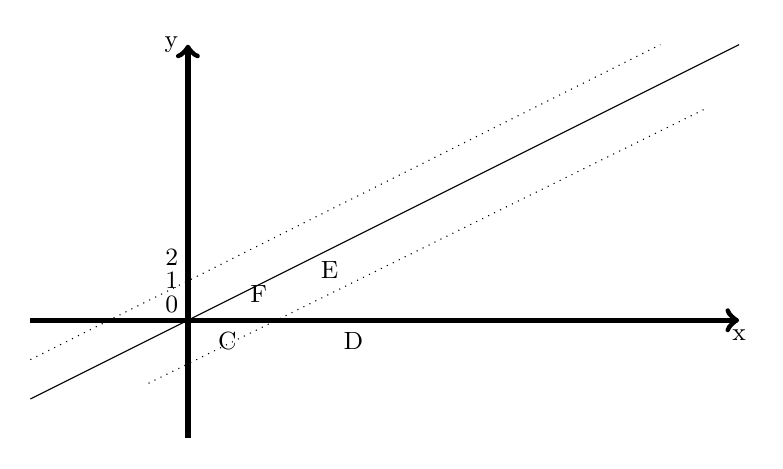
\begin{tikzpicture} [scale = 1]
\coordinate [label=left:\small{y}] (y) at (-3, 4);
\coordinate [label=below:\small{x}] (x) at (4, 0.5);
\coordinate [label=above:\small{C}] (C) at (-2.5, 0);
\coordinate [label=above:\small{D}] (D) at (-0.9, 0);
\coordinate [label=above:\small{E}] (E) at (-1.2, 0.9);
\coordinate [label=above:\small{F}] (F) at (-2.1, 0.6);
\coordinate [label=left:\small{0}] (0) at (-3, 0.7);
\coordinate [label=left:\small{1}] (1y) at (-3, 1);
\coordinate [label=left:\small{2}] (2y) at (-3, 1.3);
\draw[->, line width=2pt] (-5, 0.5) -- (4, 0.5);
\draw[->, line width=2pt] (-3, -1) -- (-3, 4);
\draw (-5, -0.5) -- (4, 4);
\draw[dotted] (-5, 0) -- (3, 4);
\draw[dotted] (-3.5, -0.3) -- (3.6, 3.2);
\end{tikzpicture}
\end{center}

\newpage
%                                  62
Ведя речь об оценке универсальных выражений, справочник говорит\linebreak
в абзаце 4.10(4) ARM\footnote{
Ada Reference Manual, имеется перевод на русский язык: см. [186]. $-$\linebreak
\textit{Прим. перев.}
}:\newline
\hspace*{25pt}"$...Furthermore,$ $if$ $a$ $universal$ $expression$ $is$ $a$ $static$ $expression$,\newline
\hspace*{15pt}$then$ $the$ $evaluation$ $must$ $be$ $exact."$\footnote{
<<... Более того, если универсальное выражение $-$ статическое, то выраже-\linebreak
ние также должно быть точным.>> см. абзац 4.10.(4) в переводе ARM ([186]).$-$\linebreak
\textit{Прим. перев.}
}
\begin{center}
\textit{Статическая проверка непростоты $F_5$}
\end{center}
\begin{lstlisting}[mathescape=true, language=Ada]
with $Text\_IO$; use $Test\_IO$;
procedure $Test\_Format\_s\_Number$ is
 $n : $ constant $:= 5$; $F_n :$ constant $:= 2 \ast\ast(2\ast\ast{n})+1$;--4_294_967_297
 
 $x_0 :$ constant $:= 5$; $x_1 :$ constant $:= (x_0 \ast\ast (2\ast\ast{6}))$
            mod $F_n$; -- $5 \ast\ast (2\ast\ast{6})$
 $x_2 :$ constant $:= (x_1 (\ast\ast 6))$ mod $F_n$; -- $5 \ast\ast (2\ast\ast{12})$
 $x_3 :$ constant $:= (x_2 (\ast\ast 6))$ mod $F_n$; -- $5 \ast\ast (2\ast\ast{18})$
 $x_4 :$ constant $:= (x_3 (\ast\ast 6))$ mod $F_n$; -- $5 \ast\ast (2\ast\ast{24})$
 $x_5 :$ constant $:= (x_4 (\ast\ast 7))$ mod $F_n$; -- $5 \ast\ast (2\ast\ast{31})$

begin
 if $x_5=F_{n-1}$ then $Put\_Line $("F_5 простое");
 else $Put\_Line$ ("F_5 составное");
 end if;
end $Test\_Fermat\_s_Number$;
\end{lstlisting}
\hspace*{15pt}Отличительная  черта  этой  программы  заключается  в  том,  что  вы-\linebreak
числения  выполняются  в  описательной  части  программы,  с  использо-\linebreak
ванием  универсальных  целых  констант  (а  не  типизированных  целых\linebreak
констант).  Именно  при  компиляции,  а  не  во  время  выполнения,  оце-\linebreak
ниваются  все  выражеция.  По  вполне  понятным  причинам  невозможно\linebreak
прямо  вычислить $5^{\frac{F_5-1}{2}}$,  а  потом  взять  остаток  по  модулю  $F_5$ (кстати,\linebreak
сколько  десятичных  цифр  содержит  число  $5^{\frac{F_5-1}{2}}$?).  Итак,  вычисление\linebreak
разбито  на  части,  используя  статическую  и  улучшенную  версию  ди\linebreak
хотомического  возведения  в  степень.  Следовательно,  выполнение  про-\linebreak
граммы ограничивается обработкой результатов, полученных при ком-\linebreak
пиляции.
\begin{mynotice}
Помимо прочего, этот пример показывает, что лю-\linebreak
бой компилятор языка Ада обладает встроенным калькулятором\linebreak
произвольно большой точности (с точностью в пределах возмож-\linebreak
ностей конкретной машины), и можно только сожалеть, что этот\linebreak
\newpage
\noindent
калькулятор  не  доступен  при  выполнении  программ.  Разумеет-\linebreak
ся, таким способом можно проверить непростоту некоторых дру-\linebreak
гих чисел Ферма, если разлагать вычисления так тщательно, что-\linebreak
бы избежать  переполнения  разрядной  сетки компилятора  (числа\linebreak
Ферма растут  очень  быстро!)
\end{mynotice}
%                                  63
\section{4 Хорошее приближение к бесконечности}
\noindent
Все задачи в информатике можно условно разделить на два класса: за-\linebreak
дачи, имеющие решение, вычисляемое за разумное время, и задачи, ре-\linebreak
шение которых требует слишом большого времени вычисления. Изуче-\linebreak
ние многочисленных классов программ (или задач) составляет особую,\linebreak
самостоятельную область информатики,  названную \textit{теорией сложно-}\linebreak
\textit{сти} (книга D. Harel, $Algorithmics: The spirit of computing$
\footnote{
Д. Харел, Алгоритмика: Дух вычислений (англ.) $-$ \textit{Прим. перев.}}$-$ это увле-\linebreak
кательнейшее введение в эту теорию). Цель этого раздела $-$ доказать,\linebreak
что  некоторые  решения  простых  математических  задач  выходят  за\linebreak
рамки возможностей современных машин. Не делая чрезмерных обоб-\linebreak
щений, можно все же сказать, что эти решения никогда не будут вычи-\linebreak
сляться на машине, какой бы она ни была! Чтобы проиллюстрировать\linebreak
этот факт,  мы  решили  реализовать  вычисление  целочисленных  опре-\linebreak
делителей при помощи метода, исходящего прямо из математического\linebreak
определения детерминанта\footnote{
Впрочем, метод, вполне применимый (хотя, может быть, правильнее было бы\linebreak
сказать неприменимый) к вычислениям детерминантов, какова бы ни была природа\linebreak
элементов, т.е. для любого базового кольца.}. Итак, вот определение детерминанта, ко­
торое будет использоваться в этом разделе.
\begin{determ}
\hspace*{15pt}Пусть $A=(a_{ij})_{\substack{1\leqslant{i}\leqslant{n}\\1\leqslant{j}\leqslant{n}}}$ $-$ квадратная матрица с целыми элемен-\linebreak
тами. Детерминант (определитель) матрицы $A$, обозначаемый $|A|$ или\linebreak
$det{A}$ $-$ это число, определенное через $|A|=\sum_{\sigma\in{S_n}}\epsilon(\sigma)a_{1{\sigma(1)}}a_{2\sigma(2)}...$\linebreak
$a_{n\sigma(n)}$, где $S_n$ $-$ это множество перестановок интервала $[1,n]$, а $\epsilon$ $-$\linebreak
функция, дающая знак перестановки.
\end{determ}
Это определение  обладает  некоторой  инвариантной  эффективно-\linebreak
стью (по крайней мере, внешне): действительно, определитель, кажет-\linebreak
ся, может быть вычислен при помощи конечной суммы, любимой опера-\linebreak
ции в программах. Однако, прежде, чем приступить к программирова-\linebreak
нию этого метода, можно, а любой разумный человек должен, задать се-\linebreak
бе вопрос: сколько слагаемых имеет эта сумма? Математик тотчас же\linebreak
\newpage
%                                  64
\noindent
ответит: в этом выражении имеется, очевидно, $n!$ слагаемых (каждое\linebreak
состоит из $n$ множителей)! И обсуждение закончено. Но кто знает, ка-\linebreak
ково значение $n!$, когда $n$ принимает значения  10, 20, ..., т.е. значения\linebreak
очень скромные для любой  практической задачи,  имеющей матричное\linebreak
решение  (например,  задачи  метеорологии  или  моделирования течения\linebreak
жидкостей, где нередко приходится оперировать матрицами, имеющи-\linebreak
ми  тысячи  строк  и  столбцов)?  И  снова  математик  может  ответить,\linebreak
используя приближение Стирлинга, что
\begin{center}
$n!\approx n^ne^{-n}\sqrt{2\pi n}$ и даже $n!>n^ne^{-n}\sqrt{2\pi n}$,
\end{center}
а любая хорошая система алгебраического вычисления дает точные ре-\linebreak
зультаты:
\begin{center}
$10!=3 628 800$ и $20!=2 432 902 008 176 640 000$.
\end{center}
Последнее значение производит некоторое впечатление, оно приблизи­-\linebreak
тельно равно $2*10^{18}$. Зная, что современные микро-ЭВМ способны со-\linebreak
вершать  около  миллиона  сложений  в  секунду,  естественно  спросить:\linebreak
сколько времени затратит такой компьютер, чтобы выполнить $2*10^{18}$\linebreak
сложений?\newline
\hspace*{15pt}Этот пример без дополнительных выкладок не убеждает скептиков,\linebreak
которые считают,  что  стали  жертвами  фокуса.  Вот  по этой  причине\linebreak
мы и решили практически доказать сложность таких программ, взяв в\linebreak
качестве примера вычисление определителя.
\subsection{4.1 Элементы обработки массивов в языке Ада}
\noindent
Матрицы  обычно  представлены  в  алгоритмах  и  программах с  помо-\linebreak
щью массивов  (если  речь  не  идет о разреженных  матрицах,  для кото-\linebreak
рых в большинстве случаев представление оптимизируют). Кроме того,\linebreak
как мы увидим  в дальнейшем,  перестановки тоже можно представить\linebreak
с помощью этой структуры.  Следовательно, нужно изучить обработку\linebreak
массивов в языке Ада.\newline
\hspace*{15pt}Обработка массивов в языке Ада имеет только отдаленное отноше-\linebreak
ние к обработке, которую можно сделать в классических языках, таких\linebreak
как Паскаль, а средства, предоставленные в распоряжение пользовате-\linebreak
ля  разработчиками  языка,  удовлетворяют все  его  (разумные)  ожида­-\linebreak
ния.  Хотя  в  языке  Ада  и  невозможно  определить  массив  переменно-\linebreak
го размера, но существует понятие, позволяющее обрабатывать массив\linebreak
неизвестного  размера  во  время  построения  программы:  это  понятие\linebreak
\textbf{шаблона} (\textit{pattern} в англосаксонской терминологии).
\newpage
%                                  65
В качестве первой иллюстрации принципа шаблонов мы покажем,\linebreak
как в языке Ада построить процедуры или функции, число аргументов\linebreak
которых кажется переменным. Этот метод использования шаблонов не\linebreak
очень принят,  но дает блестящие результаты в задачах такого вида\linebreak
(см.  работу Буха [27]).  Выбранный нами этого пример является по-\linebreak
строением функции, позволяющей находить ее  наибольший аргумент\linebreak
(среди любого их количества). Для начала рассмотрим массив,  в ко­-\linebreak
тором множество индексов (подынтервал целых положительных чисел)\linebreak
и тип основных элементов произвольны. Массив называется $T$, а тип\linebreak
элементов массива $-$ $Object$. Так как мы ничего не знаем о типе элемен-\linebreak
тов, то если мы хотим вычислить максимум элементов массива, нужно\linebreak
располагать оператором сравнения; этот оператор обозначен <<$<$>>. Вы-\linebreak
числяемое значение $Max$ должно удовлетворять условию:
\begin{center}
при любом индексе $i$ массива $T$: $T(i)=Max$ или $T(i)<Max$.
\end{center}
В этом  выражении  внимательный  читатель  отметит  использование\linebreak
двух операторов,  <<$=$>>  и  <<$<$>>,  а не единственного оператора <<$\leqslant$>>:  про-\linebreak
граммистская шероховатость, которая будет сглажена при реализации\linebreak
этой функции в языке Ада.  Алгоритм вычисления  максимума очень\linebreak
прост, и нет необходимости его подробно объяснять. Итак, предлага-\linebreak
ем сразу реализацию этой функции в языке Ада, учитывая тот факт,\linebreak
что единственные допустимые операции на элементах типа $Object$ $-$\linebreak
это: описание, присваивание и сравнение оператором <<$<$>>.
\begin{lstlisting}[mathescape=true, language=Ada, frame=none, xleftmargin=20pt]
function $Max (T : Objects\_Array)$ return $Object$ is
 $Temporary\_Maximum : Object := T (T`First)$;
begin
 for $i$ in $T`First+1 .. T`Last$ loop
  if $Temporary\_Maximum<T(i)$ then $Temporary\_Maximum := T(i)$;
  end if;
 end loop;
 return $Temporary\_Maximum$;
end $Max$;
\end{lstlisting}
Основная характеристика этой части Ада-программы $-$ это полное от-\linebreak
сутствие явной ссылки на любое особое свойство обрабатываемого мас-\linebreak
сива: точно не известно, каковы индексы массива, и также не известны\linebreak
элементы, составляющие массив, а единственные используемые опера-\linebreak
ции $-$ это три операции, названные выше. Однако можно обработать\linebreak
массив, обработать его границы благодаря предопределенным функ-\linebreak
циям в языке Ада, которые называют \textit{атрибутами}. Таким образом,\linebreak
если $T$ $-$ массив, выражение $T`First$ обозначает наименьший  индекс\linebreak
массива $T$, a $T`Last$ обозначает наибольший индекс $T$. Это доказыва-\linebreak
\newpage

%                                  66
\noindent
ет, что функция, имеющая массив в качестве формального параметра,\linebreak
может каждый раз заново определять некоторые характеристики мас-\linebreak
сива,  который ей  передан  в качестве фактического параметра (длина,\linebreak
границы...):  атрибуты позволяют определить эти характеристики \textit{ди}-\linebreak
\textit{намически}, т.е. во время выполнения. Хотя это явно не выражено, но в\linebreak
этой  функции  используется  особое  свойство  индексов:  их  целочислен-\linebreak
ный характер, который позволяет записать выражение $T`First+1$.\newline
\hspace*{15pt}Логическое  следствие  всего  этого  заключается  в  том,  что  текст\linebreak
функции $Max$ всегда один и тот же и что обрабатываемые объекты $-$\linebreak
это  целые  числа,  действительные  числа,  литералы  перечисления  или\linebreak
любой другой объект при условии,  что пользователь задаст операцию\linebreak
сравнения. Другими словами, очень легко записать на основе всего ска-\linebreak
занного настраиваемый алгоритм вычисления максимума. Таким обра-\linebreak
зом, спецификация, обозначения которой слегка отличаются от преды-\linebreak
дущих, выглядит так:
\begin{center}
\textit{Спецификация настраиваемого алгоритма вычисления максимума}
\end{center}
\begin{lstlisting}[mathescape=true, language=Ada]
generic
    type $Object$ is private;
    with $Function "<" (a,b : Object)$ return $Boolean$ is $<>$;
package $Maximum$ is
    type $Objects\_Array$ is array $(Positive$ range $<>)$ of $Object$;
    function $Max (T : Objects\_Array)$ return $Object$;
end $Maximum$;
\end{lstlisting}
\hspace*{15pt}Рассмотрим сначала формальные  параметры  настройки  для этого\linebreak
пакета. Тип $Object$ $-$ это приватный тип; это означает, как мы видели\linebreak
в  разделе  3.3  (стр.  53),  что  единственными  операциями,  допустимы-\linebreak
ми неявно внутри пакета на объектах этого типа, являются описание,\linebreak
присваивание,  тест  на  равенство  и  использование  в  качестве  параме-\linebreak
тра  подпрограммы.  Следовательно,  разработчик  функции $Max$ ниче-\linebreak
го  не  знает  о  типе $Object$; он  не  может знать,  идет  ли  речь  о  целом\linebreak
типе,  последовательности  знаков...  Второй  формальный  параметр $-$\linebreak
это оператор сравнения элементов типа $Object$, необходимый для вычи-\linebreak
сления максимального значения,  но который невозможно прямо ввести\linebreak
из-за  незнания  типа $Object$. Кроме  того,  этот  формальный  параметр\linebreak
настройки  имеет  значение  по  умолчанию;  описание $\blacktriangleright$ \textbf{with function}\linebreak
$"<" (a,b : Object)$ \textbf{return} $Boolean$ is $<>; \blacktriangleleft$ означает,  что в случае,  ко-\linebreak
гда пользователь настраиваемого пакета не задает явно эту  функцию\linebreak
в момент конкретизации, то функция, которая должна быть использо-\linebreak
вана, — это функция $<$, имеющая соответствующий тип параметров и\linebreak
видимая в  месте  конкретизации.  Формальным параметрам настройки\linebreak
\newpage
%                                  67
\noindent
могут быть заданы другие виды значений по умолчанию, в дальнейшем\linebreak
мы еще с ними встретимся.\\

Имея эти два параметра, разработчик функции $Max$ задает пользо-\linebreak
вателю, с одной стороны, тип $Objects\_Array$, который, в основном, не\linebreak
будет использоваться,  и функцию $Max$, которая нас интересует.  Тип\linebreak
$Objects\_Array$ служит только для описания типа параметров функции\linebreak
$Max$. Как будет видно в применении функции, пользователь может его\linebreak
полностью игнорировать. Описание типа $Objects\_Array$ $-$ это несколько\linebreak
своеобразное описание массива: $\blacktriangleright$ \textbf{type} $Objects\_Array$ \textbf{is array} $(Positive$\linebreak
\textbf{range}<>$)$ \textbf{of} $Object;\blacktriangleleft$. Это будет точное описание шаблона, и говорить\linebreak
о типе, имеющем отношение к идентификатору $Object\_Array$, значит\linebreak
злоупотреблять языком. Действительно, невозможно описать перемен-\linebreak
иые типа $Object\_Array$, потому что Ада, как любой другой язык, дол-\linebreak
жен иметь возможность предоставить в памяти место, необходимое для\linebreak
массива. Впрочем, вполне возможно использовать этот шаблон для опи-\linebreak
сания типа формальных параметров подпрограммы: при фактическом\linebreak
использовании подпрограммы ее параметрами будут описанные пере-\linebreak
менные (обратное было бы удивительным) или выражения, построен-\linebreak
ные в момент вызова, характеристики которых хорошо известны, когда\linebreak
контроль идет внутри подпрограммы.\\

Тело пакета $Maximum$ записывается прямо, непосредственно и явля­-\linebreak
ется, по существу, ни чем иным, как переформулировкой функции $Max$,\linebreak
представленной выше.
\begin{center}
\textit{Реализация функции Max}
\end{center}
\begin{lstlisting}[mathescape=true, language=Ada, xleftmargin=15pt]
package body $Maximum$ is
 function $Max (T : Objects\_Array)$ return $Object$ is
  $Temporary\_Maximum : Object := T (T`First)$;
 begin
  for $i$ in $T`First+1 .. T`Last$ loop
   if $Temporary\_Maximum < T(i)$ then $Temporary\_Maximum := T(i);$ end if;
  end loop;
 return $Temporary\_Maximum$;
 end $Max$;
end $Maximum$;
\end{lstlisting}
\hspace*{15pt}Перейдем теперь к использованию этой функции. Неинтересно по-\linebreak
дробно объяснять всю программу, использующую эту функцию (в са-\linebreak
мом деле, длина такой программы была бы огромной по сравнению с\linebreak
необходимым пояснением функции $Max$), однако несколько фрагментов\linebreak
такой программы разъяснят возможности функции.
\newpage
%                                  68
\begin{lstlisting}[mathescape=true, language=Ada, frame=none, xleftmargin=15pt]
with $Maximum;--$ Продолжение контекста компиляции
procedure $Using\_Function\_Max$ is
 type $My\_Integer$ is $...-- \text{ В этом месте уже определен оператор "<"}$
                         $\text{на целых числах типа Integer}$
 package $Integer\_Maximum$ is new $Maximum (My\_Integer)$;
                         use $Integer\_Maximum$;
 $x , a , b , c , d : My\_Integer;--\text{Продолжение описаний(переменные ...)}$
begin
 $--\text{ Начало вычислений}$
 $x := Max ((a,b,c));--\text{ Продолжение вычислений}$
 $x := Max ((a,b,c,d));--\text{ Конец вычислений}$
end $Using\_Function\_Max$;
\end{lstlisting}
\hspace*{15pt}Эта программа использует конкретизацию пакета $Maximum$ для це-\linebreak
лых чисел; как видим, она начинается с оператора контекста (может\linebreak
быть неполного в примере), ссылающегося на настраиваемый пакет.\linebreak
Внутри главной процедуры после определения  целого типа, который\linebreak
наследует обычные операции на целых числах, и в частности, опера-\linebreak
тор сравнения <<$<$>>, находим конкретизацию настраиваемого пакета, в\linebreak
которой задан только фактический параметр, соответствующий типу\linebreak
$Object$; так как второй параметр явно не задан, при конкретизации для\linebreak
него используется значение по умолчанию, т.е. стандартный оператор\linebreak
<<$<$>> сравнения целых чисел. Можно уже заметить, что если бы вместо\linebreak
использования оператора <<$<$>> передали  в качестве второго параметра\linebreak
оператор <<$>$>>, как в команде
\begin{lstlisting}[mathescape=true, frame=none, language=Ada, xleftmargin=15pt]
package $Integer\_Minimum$ is new $Maximum (My\_Integer, ">")$;
\end{lstlisting}
то построенная таким образом функция $Max$ вычислила бы наименьший\linebreak
из своих аргументов, а не наибольший.\newline
\hspace*{15pt}После спецификатора видимости $\blacktriangleright$ \textbf{use} $Integer\_Maximum \blacktriangleleft$ и не-\linebreak
скольких дополнительных описаний находим тело главной процедуры,\linebreak
которое содержит определенное количество дополнительных вычисле-\linebreak
ний и (что нас интересует) два обращения к функции $Max$:
\begin{lstlisting}[mathescape=true, language=Ada, frame=none, xleftmargin=15pt]
$x:=max ((a,b,c)); x:=max ((a,b,c,d))$;
\end{lstlisting}
Выражения,  которые  образуют  фактические  параметры  этих  двух\linebreak
обращений,  являются \textit{агрегатами}, т.е.  явными  структурными\linebreak
конструкциями.  Фактический  параметр первого обращения  к функ-\linebreak
ции $Max$ $-$ это агрегат $(a,b,c)$, который вне своего контекста пред­-\linebreak
ставляет структуру с тремя компонентами типа $My\_Integer$. Это вы-\linebreak
ражение  (агрегат) совместимо с точки зрения типа как с записью с\linebreak
тремя полями типа $My\_Integer$, так и с индексируемым типом с тремя\linebreak
компонентами,  индексы  которого абсолютно произвольны.  Контекст\linebreak
\newpage
%                                  69
\noindent
использования  этого  агрегата  определяет  точным  образом  тип  выра-\linebreak
жения $(a,b,c)$: так как это параметр функции $Max$, то мы имеем  дело с\linebreak
индексируемым  типом  с  тремя  компонентами  (потому  что  в  агрегате\linebreak
их три),  индексированным посредством подынтервала типа $Positive$. О\linebreak 
нем  больше  ничего  не  известно,  и  точное  определение  данного  интер-\linebreak
вала  не  представляет  здесь  никакого  интереса  (за  дополнительными\linebreak
сведениями читатель может обратиться к $ARM$). В этих условиях вто-\linebreak
рой  вызов  функции $Max$ существенно  не  отличается  от  первого:  эта\linebreak
функция  может  применяться  к  массивам  любой  длины,  и  если  бы  не\linebreak
перегруженность  скобками,  то  можно  было  бы  сказать,  что  функция\linebreak
$Max$ обладает переменным  числом  параметров.\newline
\hspace*{15pt}Теперь  должно быть ясно,  что  пользователю этой  функции  нет  не-\linebreak
обходимости представлять тип $Objects\_Array$ в программе; один из слу-\linebreak
чаев, когда это будет необходимо, соответствует использованию функ-\linebreak
ции $Max$, применяемой к \textit{переменной} индексируемого  типа,  но это уже\linebreak
другая  история...
\subsection{4.2 Работа с матрицами}
\noindent
Следующий этап обучения обработке массивов в языке Ада заключает-\linebreak
ся  в  изучении  представления  матриц,  базовых операций  над  матрица-\linebreak
ми,  ввода-вывода  матриц  $-$  короче,  в  определении  так  называемого\linebreak
\textbf{абстрактного  типа  данных} и  в  построении  нескольких  средств\linebreak
управления  такого типа.\newline
\hspace*{15pt}Первая  фаза $-$  определение  абстрактного  типа  данных $-$ начина-\linebreak
ется с распознавания того, что называют простейшими  операциями на\linebreak
типе.  Сначала можно отметить,  что эти  операции  подразделяются  на\linebreak
два вида: \textbf{конструкторы } и \textbf{селекторы}\footnote{
Эта терминология кажется повсюду принята программистами, она произо-\linebreak
шла из разработки технологии программного обеспечения. Можно обратиться к\linebreak
книге Буха $[27]$, которая дает более полные определения с последующим стилем\linebreak
программирования.}. Конструкторы $-$ это опера-\linebreak
ции,  которые  модифицируют состояние  (значение)  данных,  тогда как\linebreak
селекторы  позволяют только узнать это состояние.\newline
\hspace*{15pt}Каковы  же  будут фундаментальные операции,  когда объект $-$  ма-\linebreak
трица?  Прежде  всего,  имеется  конструктор,  который  позволяет  при-\linebreak
сваивать значение элементу матрицы,  а также симметричная операция\linebreak
селектор,  позволяющий  узнать  значение  одного  из  элементов.  Напри\linebreak
мер,  если $A - $ рассматриваемая  матрица,  а $a_{ij}-$ интересующий  нас\linebreak
элемент, то обычно обозначаем $A(i,j)\longleftarrow v$ и $v\longleftarrow A(i,j)$ те действия,\linebreak
которые реализуют эти операции. Но такой способ действия имеет мно-\linebreak
\newpage

%                                  70
\noindent
го последствий и, в частности, приводит к тому, что матрицы всегда\linebreak
представляются с помощью массивов. Однако хорошо известно, что это\linebreak
не так! Некоторые матрицы $-$ разреженные: матрицы, у которых толь-\linebreak
ко небольшое количество элементов не равно нулю; было бы совершенно\linebreak
неразумно, с точки зрения информатики, представлять матрицу боль-\linebreak
ших размеров, например, $1000\times 1000$, с помощью массива в миллион\linebreak
клеток, если всего лишь 10000 элементов не равны нулю. Следователь-\linebreak
но,  если  все  программы,  составленные  для  работы  с  матрицами, ис-\linebreak
пользуют понятие индексируемого типа, то эти программы становятся\linebreak
полностью непригодными, когда хотят применить их алгоритмы к раз-\linebreak
реженным матрицам. Иначе говоря, программы слишком зависимы от\linebreak
внутреннего представления обрабатываемых объектов.\newline
\hspace*{15pt}Конкретно, этот тип  представления обязывает программиста вы-\linebreak
ражать присваивание и оценку элемента матрицы, соответственно, по-\linebreak
средством вызова процедуры и функции, даже если это, возможно, бу-\linebreak
дет тяжелее записывать (что справедливо лишь отчасти). Конструктор\linebreak 
обозначен $Set\_Coefficient$, а селектор $- Coefficient\_Of$ со спецификаци-\linebreak
ями, которые мы увидим в пакете, представленном далее.\newline
\hspace*{15pt}Этих двух операций недостаточно, чтобы выполнить все возможные\linebreak
манипуляции на матрице; не хватает селекторов, позволяющих узнать\linebreak
размер матриц, чтобы знать, какие элементы существуют. Так как тон-\linebreak
кая структура матрицы совершенно не известна пользователю матрицы\linebreak
(но не разработчику, роль которого мы сейчас выполняем), невозможно\linebreak
использовать различные атрибуты массива, как в предыдущем разделе\linebreak
а нужно явно задать функции, позволяющие оценить границы матри-\linebreak
цы: $First\_Row, Last\_Row, First\_Column, Last\_Column$.\newline
\hspace*{15pt}Чтобы модуль был как можно более автономным, нужно предусмо-\linebreak
треть  и  классифицировать  возможные ошибки  и  сопоставить им ис-\linebreak
ключения.  В случае матрицы единственная ошибка обработки $-$ это\linebreak
ссылка  на  несуществующий  элемент;  эту  ошибку  символизирует  ис-\linebreak
ключение $Index\_Out\_Of\_Bounds$, которое может появиться только при\linebreak
выполнении простейших операций $Set\_Coefficient$ и $Coefficient\_Of$.\newline
Вот полная спецификация настраиваемого пакета, реализующего аб-\linebreak
страктный тип данных.
\begin{center}
\textit{Матрица с целыми элементами}
\end{center}
\begin{lstlisting}[mathescape=true, language=Ada, frame=lrt]
generic
 type $Row\_Index$ is range <>;
 type $Column\_Index$ is range <>;
 type $Coefficient$ is range <>;
\end{lstlisting}
\newpage
%                                  71
\begin{lstlisting}[mathescape=true, language=Ada, frame=lbr]
package $Matrix\_Nonsparse\_Integer$ is
 type $Matrix (First\_Row : Row\_Index; Last\_Row : Row\_Index;$
      $First\_Column : Column\_Index; Last\_Column : Column\_Index)$ is private;
 procedure $Set\_Coefficient (Of\_The\_Matrix :$ in out $Matrix$;
                     $At\_Row :$ in $Row\_Index$;
                     $And\_Column :$ in $Column\_Index$;
                     $To\_The\_Value :$ in $Coefficient)$;
 function $Coefficient\_Of (The\_Matrix : Matrix$;
                     $At\_Row : Row\_Index$;
                     $And\_Column : Column\_Index)$ return $Coefficient$;            
 function $First\_Row (Of\_The\_Matrix : Matrix)$ return $Row\_Index$;
 function $Last\_Row (Of\_The\_Matrix : Matrix)$ return $Row\_Index$;
 function $First\_Column (Of\_The\_Matrix : Matrix)$ return $Column\_Index$;
 function $Last\_Column (Of\_The\_Matrix : Matrix)$ return $Column\_Index$;
 
 $Index\_Out\_Of\_Bounds :$ exception;
 
private
 type $Matrix\_Template$ is
     array$(Row\_Index$ range <>,$Column\_Index$ range <>$)$ of $Coefficient$;
 type $Matrix (First\_Row : Row\_Index; Last\_Row : Row\_Index;$
            $First\_Column : Column\_Index; Last\_Column : Column\_Index)$
 is record
  $The\_Coefficient :$
     $Matrix\_Template (First\_Row .. Last\_Row, First\_Column .. Last\_Column)$;
 end record;
 pragma $Inline (Set\_Coefficient, Coefficient\_Of,$
             $First\_Row, Last\_Row, First\_Column, Last\_Column)$;
end $Matrix\_Nonsparse\_Integer$;
\end{lstlisting}

Первое замечание касается имени пакета, $Matrix\_Nonsparse\_Integer$.\linebreak
В  этом  имени  соблюдаются  простейшие  правила  построения:  первый\linebreak
радикал означает,  что  абстрактный  тип  данных,  который в  нем  опре-\linebreak
делен, $-$ матрица, второй, что эти матрицы не разреженные  (алгорит-\linebreak
мы  доступа  к  разреженным  матрицам,  в  основном,  другие),  и,  нако-\linebreak
нец, суффикс указывает на тип элементов. Это имя позволяет сразу же\linebreak
узнать примерные характеристики  определенного объекта\footnote{
Эта  проблема  может  показаться  устаревшей,  но  в  программировании  выбор\linebreak
идентификаторов $-$ важная и  тонкая операция, и  некоторые труды по  разработке\linebreak
технологии программного обеспечения посвящают этой проблеме целую  главу.}.\newline
Рассмотрим теперь видимую часть этой спецификации  (т.е.  все то,\linebreak
что предшествует  ключевому слову \textbf{private}). Прежде  всего,  формаль-\linebreak
%                                  72
\noindent
ных параметров  настройки  три  и  их  семантика  должна  быть ясной...\linebreak
Читатель педантичный  (и усидчивый, см. раздел 3.3) сможет нас упрек­-\linebreak
нуть  в  том,  что мы  не  определили,  что элементы  — личного типа  (т.е.\linebreak
почти  любого),  это  позволило  бы  обрабатывать одинаковым  способом\linebreak
матрицы  целых  чисел,  чисел  с  плавающей  запятой,  многочленов и  т.д.\linebreak
Этот выбор  основан  на  том,  что  обычно  не  совершают  один  и  тот же\linebreak
тип  вычислений  и  на матрицах с целыми  и  на  матрицах с  действитель­-\linebreak
ными  элементами  и  что  алгоритмы  вычисления  на  матрицах  много­-\linebreak
членов  не являются  простым  применением  в  кольце  многочленов  алго­-\linebreak
ритмов  для  матриц  с  элементами  из  числового  кольца.  Другими  сло­-\linebreak
вами,  алгоритмы  вычисления  на  алгебраических  структурах  соответ­-\linebreak
ствуют  структурному  типу,  который  подлежит  обработке.  Например,\linebreak
если $A-$ матрица и  если a мы хотим вычислить $A^n$,  то  для этого можно\linebreak 
взять  великолепную  настраиваемую  функцию  дихотомического  возве­-\linebreak
дения в степень,  изученную в разделе 3.3; но намного более экономично,\linebreak
при условии,  что $n-$ достаточно большое, вычислить характеристиче-\linebreak
ский  многочлен (или  минимальный,  если  умеем  его  вычислять) от $A$  и\linebreak 
прежде,  чем  вычислить  произведения  матриц,  привести  $A^n$  по  модулю \linebreak
этого  многочлена.  Все  эти  примеры  показывают,  что  можно  фиксиро­-\linebreak
вать  тип  элементов  матрицы:  что  теряем  в  общем,  то  выигрываем  в\linebreak
полезном...\\

Собственно  спецификация  начинается  с  определения  личного  типа\linebreak
$Matrix$, который обладает четырьмя дискриминантами с красноречивы-\linebreak
ми  именами.  Когда этот пакет  получит  начальные значения, тогда бу-\linebreak
дет возможно описать, например, переменную $\blacktriangleright A:Matrix(2,4,3,7);\blacktriangleleft$
это  означает,  что  $A-$ это  матрица  $3\times 5$,  у  которой  индексы  строчек\linebreak 
находятся  в  интервале  $[2,4]$,  а  индексы  столбцов  $-$  в  интервале  $[3,7]$.\linebreak 
Конкретизация  этого  пакета  порождает  не  единственный  матричный\linebreak
тип, а, скорее,  класс матриц, имеющих некоторые общие характеристи-\linebreak
ки  (тип  индексов  и  конкретный  тип  элементов).  Преимущество  этого\linebreak
способа  действия  состоит  в  том,  что  он  позволяет  обрабатывать  ма-\linebreak
трицы  различных  размеров,  исходя  только из  начальных значений.\\

Перейдем  теперь  к  точному  определению  типа $Matrix-$ определе-\linebreak
нию,  которое  обычному,  среднему  пользователю знать  необязательно.\linebreak 
Так  как  реализуются  <<полные>>  матрицы,  внутреннее  представление  ис-\linebreak
пользует  двумерные  массивы.  Но  синтаксис  языка  Ада  предписывает,\linebreak
чтобы  определение  типа,  фигурирующее  в  личной  части,  имело  то же\linebreak
начало,  что присутствует  у  него  в спецификации.  Следовательно, этот\linebreak
тип  должен  быть  типом  дискриминанта  записи,  его  единственное  по-\linebreak
ле  (отличное от  дискриминантов)  $-$ это двумерный  массив,  о котором\linebreak
\newpage

